\chapter{Circles}

A circle is the set of points $(x, y)$ that are a particular distance $r$ from a
particular point $(x_c, y_c)$.  We say that $r$ is the
\newterm{radius} and $(x_c, y_c)$ is the \newterm{center}

\begin{tikzpicture}
    \filldraw [sdkblue] (1,2) circle (2pt) node[anchor=west]{$(x_c, y_c)$};
    \filldraw [sdkblue] (2,4.82842712474619) circle (2pt) node[anchor=west]{$(x, y)$};
    \draw [sdkblue,dashed](1,2) -- (2,4.82842712474619) node[midway,anchor=west] {$r$};
    \draw [sdkblue](1,2) circle (3);
    \draw [stealth-stealth](-2.5,0)--(4.5,0);
    \draw [stealth-stealth](0,-1.5)--(0,5.5);
\end{tikzpicture}

\begin{mdframed}[style=important, frametitle={Area and Radius}]

  If the radius of a circle is $r$, the area of its interior ($a$) is given by \index{circle!area of}

  $$a = \pi r^2$$

\end{mdframed}

\begin{Exercise}[title={Area of a Circle}, label=area_of_circle]

  The paint you have says ``One liter covers 6 square meters.''

  You are painting the top of a circular table with a radius of 3 meters.

  How much paint will you need?
  
\end{Exercise}
\begin{Answer}[ref=area_of_circle]

  The table has a radius of 3 meters.

  So the area of its top is $3^2 \pi \approx 28.27$.

  $$ 28.27 \text{ square meters }\left(\frac{1 \text{ liter }}{6 \text{ square meters }} \right) = 4.72 \text{ liters }$$ 
  
\end{Answer}


Note that a circle lives in a particular plane. The points $(x, y, z)$ that are a particular distance $r$ from a
particular point $(x_c, y_c, z_c)$ are a sphere:

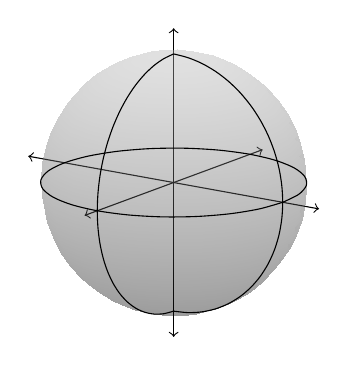
\begin{tikzpicture}
  \begin{axis}[
    view={35}{15},
    unit vector ratio=1 1 1,
    ticks = none,
    axis lines=middle,
    ymin=-3.5,
    ymax=3.5,
    xmax=4.0,
    xmin=-4.0,
    zmin=-3.6,
    zmax=3.6,
    x axis line style=<->,
    y axis line style=<->,
    z axis line style=<->,
    clip=false
    ]
    \addplot3[surf,shader=interp,domain=0:360,y domain=-90:90, opacity=0.4,
    colormap={blackwhite}{color=(black) color=(black!30)}] ({3 * cos(y) * cos(x)},
    {3 *  cos(y) * sin(x)},{3 * sin(y)});
    \addplot3[samples y=0,domain=0:360,smooth]({3*cos(x)}, {3*sin(x)}, 0.0);
    \addplot3[samples y=0,domain=-180:0,smooth](0, {3*sin(x)}, {3*cos(x)});
    \addplot3[samples y=0,domain=0:180,smooth]({3*sin(x)}, 0, {3*cos(x)});
  \end{axis}
\end{tikzpicture}

The distance all the way across the middle of a circle (or a sphere) is its
\newterm{diameter}.  The diameter is always twice the radius.

For the rest of the chapter, we are talking about circles, points, and
lines \textit{in a plane}.

\begin{mdframed}[style=important, frametitle={Circumference and Diameter}]

  The circumference ($c$) of a circle is the distance around the circle. If the diameter is $d$, \index{circumference}

  $$c = \pi d$$

\end{mdframed}

\begin{Exercise}[title={Circumference}, label=circumference]

  Using a tape measure, you figure out that the circumference of a tree in your yard is 64 cm.

  Assuming the trunk is basically circular,  what is its diameter?
  
\end{Exercise}
\begin{Answer}[ref=circumference]

  The diameter is $$\frac{c}{\pi} = \frac{64}{\pi} \approx 20.37 \text{ centimeters}$$
  
\end{Answer}
\begin{Exercise}[title={Splitting a Pie}, label=pie_splitting]

  A pie has a radius of 13 cm.  7 friends all want equal sized wedges.  You have a tape measure.

  How many centimeters will each outer crust be?

\end{Exercise}
\begin{Answer}[ref=pie_splitting]

  The circumference of the pie is $26 \pi \approx 81.7$ centimenters.
  
  The length of the crust for each piece would be about $\frac{81.7}{7} = 11.7$ cm.

  
\begin{tikzpicture}
    \filldraw [black] (0,0) circle (2pt);
    \draw [black](0,0) circle (3);
    \foreach \x in {0,...,6}
    \draw [dashed] (0,0) -- ({3 * cos(\x * 51.428571428571429)}, {3 * sin(\x * 51.428571428571429)});
    \draw [sdkblue,very thick] (3, 0) arc (0:51.43:3) node [midway, anchor=east] {11.7 cm};
    \node at (1.0, 1.5)  {13 cm};
\end{tikzpicture}
\end{Answer}



\begin{mdframed}[style=important, frametitle={Length of an Arc}]

If you have two points $a$ and $b$ on a circle, the ray from the
center through $a$ and the ray from the center through $b$ form an
angle.  If $\theta$ is the angle in radians and $r$ is the radius of
the circle, the distance from $a$ to $b$ on the circle is $r \theta$.

\begin{tikzpicture}
    \filldraw [black] (0,0) circle (2pt) node[anchor=west]{Center};
    \filldraw [sdkblue] (-1,2.82842712474619) circle (2pt) node[anchor=west]{$b$};
    \filldraw [sdkblue] (2.12132,2.12132) circle (2pt) node[anchor=east]{$a$};
    \draw [sdkblue,dashed,->](0,0) -- (-1.2,3.394112549695428);
    \draw [sdkblue,dashed,->](0,0) -- (2.4, 2.4) node[midway,anchor=east]{$r$};
    \draw [black](0,0) circle (3);
    \draw [sdkblue,very thick] (2.12132,2.12132) arc (45:109.47:3) node [midway, anchor=south] {$r \theta$};
    \draw [sdkblue, <->] (0.707,0.707) arc (45:109.47:1) node [midway, anchor=south]{$\theta$};
\end{tikzpicture}

\end{mdframed}

\begin{Exercise}[title={Arc Length}, label=arc_length]

You have been asked to find the radius of a very large cylindrical tank.
You have a tape measure, but it is only 15 meters long and doesn't
reach all the way around the tank.

However, you have a compass.  So you stick one end of the tape measure
to the side of the tank and measure the orientation of the wall at
that point.  Then you walk the 15 meters and measure the orientation of the wall there.

You find that 15 meters represents 72 degrees of arc.

What is the radius of the tank in meters?
  
\end{Exercise}
\begin{Answer}[ref=arc_length]

  $$72 \text{ degrees } \left(\frac{2\pi \text{ radians }}{360 \text{ degrees }}\right) \approx 1.2566 \text{ radians }$$

  $$15 = 1.2566r$$

  $$r = 11.94 \text{ meters}$$
  
\begin{tikzpicture}
    \filldraw [black] (0,0) circle (2pt);
    \draw [black](0,0) circle (3);
    \draw [dashed] (0,0) -- ({3 * cos(72)}, {3 * sin(72)});
    \draw [dashed] (0,0) -- (3, 0);
    \draw [sdkblue,very thick] (3,0) arc (0:72:3) node [midway, anchor=east] {15 m};
    \draw [sdkblue, <->] (1,0) arc (0:72:1) node [midway, anchor=east]{$72^\circ$ = 1.2566 rad};
    \node at (0.0, 1.6)  {11.94 m};
\end{tikzpicture}
\end{Answer}

\section{Tangents}

A line that is \newterm{tangent} to a circle touches it at exactly one point:

\begin{tikzpicture}
    \filldraw [black] (0,0) circle (2pt);
    \draw [dashed, black](0,0) circle (3);
    \filldraw [sdkblue] (2.121, 2.121) circle (2pt);
    \draw [sdkblue, thick] (6.243, -2) -- (0, 4.243);
\end{tikzpicture}

The tangent line is always perpendicular to the radius to the point of tangency:

\begin{tikzpicture}
  \filldraw [black] (0,0) circle (2pt);
  \draw [dashed, black](0,0) circle (3);
  \filldraw [sdkblue] (2.121, 2.121) circle (2pt);
  \draw [sdkblue, thick] (0,0) -- (2.121, 2.121);
  \draw [black] (1.9, 1.9) -- (2.121, 1.679) -- (2.342,1.9);
  \draw [sdkblue, thick] (6.243, -2) -- (0, 4.243);
\end{tikzpicture}


\begin{Exercise}[title={Painting a Comet}, label=painting_comet]
  
  You have been asked to paint a comet and its tail in yellow on the floor of a gymnasium.

  A liter of yellow paint covers 6 square meters.

  First you draw a circle with a radius of 3 meters.  Then you mark a
  point $D$ on the floor 7 meters from the center of the circle.  Then
  you draw two tangent lines that pass through $D$.

  You use a protractor to measure the angle at which the tangent lines meet: about $51^\circ$
  
  \begin{tikzpicture}
    \filldraw [sdkblue] (0,0) circle (2pt);
    \filldraw [black] (7,0) circle (2pt);
    \draw [sdkblue,dashed] (0,0) -- (3,0) node [midway, anchor=south] {3 m};
    \draw [sdkblue,dashed] (3,0) -- (7,0) node [midway, anchor=south] {4 m};
    \draw [sdkblue,dashed, ->] (5.5,0) arc (180:154.6:1.5) node [midway, anchor=west]{$51^\circ$};
    \draw [sdkblue,dashed, ->] (5.5,0) arc (180:205.4:1.5);
    \draw [black,thick] (7,0) -- ({3 * cos(64.62)}, {3 * sin(64.62)});
    \draw [black,thick] (7,0) -- ({3 * cos(-64.62)}, {3 * sin(-64.62)});
    \filldraw [black] ({3 * cos(64.62)}, {3 * sin(64.62)}) circle (2pt);
    \filldraw [black] ({3 * cos(-64.62)}, {3 * sin(-64.62)}) circle (2pt);
    \filldraw [sdkblue] (3, 0) circle (2pt);
    \draw [sdkblue,dashed] ({3 * cos(-64.62)}, {3 * sin(-64.62)}) arc (-64.62:64.62:3);
    \draw [black,thick] ({3 * cos(64.62)}, {3 * sin(64.62)}) arc (64.62:295.38:3);
  \end{tikzpicture}

  Before you paint the area contained by the circle and the two
  tangent lines, how much paint will you need?
    

\end{Exercise}
\begin{Answer}[ref=painting_comet]

  The trick here is to take advantage of the fact that the tangent is perpendicular to the radius to make right triangles:

  \begin{tikzpicture}
    \coordinate (a) at ({3 * cos(64.62)}, {3 * sin(64.62)});
    \coordinate (b) at ({3 * cos(-64.62)}, {3 * sin(-64.62)});
    \filldraw [sdkblue] (0,0) circle (2pt);
    \filldraw [black] (7,0) circle (2pt);
    \draw [black,thick] (0,0) -- (a) node [midway, anchor=east] {3m};
    \draw [black,thick] (0,0) -- (b) node [midway, anchor=east] {3m};
    \draw [black,thick] (0,0) -- (7,0) node [midway, anchor=south] {7 m};
    \draw [sdkblue,dashed, <->] (5.5,0) arc (180:154.6:1.5) node [midway, anchor=west]{$25.5^\circ$};
    \draw [sdkblue,dashed, <->] (5.5,0) arc (180:205.4:1.5) node [midway, anchor=west]{$25.5^\circ$};
    \draw [sdkblue,dashed, <->] (1.5,0) arc (0:64.5:1.5) node [midway, anchor=west]{$64.5^\circ$};
    \draw [sdkblue,dashed, <->] (1.5,0) arc (0:-64.5:1.5) node [midway, anchor=west]{$64.5^\circ$};
    \draw [black,thick] (7,0) -- (a);
    \draw [black,thick] (7,0) -- (b);
    \filldraw [black] (a) circle (2pt);
    \filldraw [black] (b) circle (2pt);
    \draw [black,thick] (a) arc (64.62:295.38:3);
  \end{tikzpicture}

  The wedge has radius 3 and represents $360 - 2(64.5) = 231^\circ \approx 4.03 \text{ radians}$.

  We are finding the area of this piece:
  
  \begin{tikzpicture}
    \coordinate (a) at ({3 * cos(64.62)}, {3 * sin(64.62)});
    \coordinate (b) at ({3 * cos(-64.62)}, {3 * sin(-64.62)});
    \filldraw [sdkblue] (0,0) circle (2pt);
    \draw [black,thick] (0,0) -- (a) node [midway, anchor=west] {3m};
    \draw [black,thick] (0,0) -- (b);
    \draw [sdkblue,dashed, <->] ({1.5 * cos(64.62)}, {1.5 * sin(64.62)}) arc (64.5:295.5:1.5) node [midway]{4.03 rad};
    \filldraw [black] (a) circle (2pt);
    \filldraw [black] (b) circle (2pt);
    \draw [black,thick] (a) arc (64.62:295.38:3);
  \end{tikzpicture}

  The area of this piece is $(4.03)(3^2) = 36.27$ square meters.

  If a right triangle has a hypotenuse of 7m and one leg is 3m, the
  other leg is $\sqrt{7^2 - 3^2} = 2 \sqrt{10} \approx 6.3$ m.

    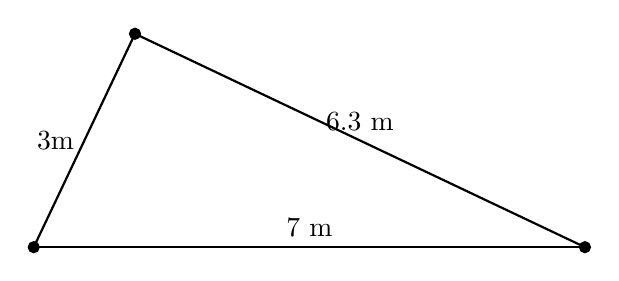
\begin{tikzpicture}
    \coordinate (a) at ({3 * cos(64.62)}, {3 * sin(64.62)});
    \filldraw [black] (7,0) circle (2pt);
    \filldraw [black] (0,0) circle (2pt);
    \draw [black,thick] (0,0) -- (a) node [midway, anchor=east] {3m};
    \draw [black,thick] (0,0) -- (7,0) node [midway, anchor=south] {7 m};
    \draw [black,thick] (7,0) -- (a) node [midway, anchor=south] {6.3 m};
    \filldraw [black] (a) circle (2pt);
  \end{tikzpicture}

  
  A right triangle with legs of 3m and 6.3m has an area of 9.45 square meters.

  There are two of them, so the total area is $36.27 + 2(18.9) = 74.07$ square meters.

  Six square meters per liter, so you need $\frac{74.07}{6} = 12.35$ liters of paint.

\end{Answer}
